\documentclass[9pt]{beamer}

% Created By Gouthaman KG

\usepackage[utf8]{inputenc}
\usepackage[T1]{fontenc}
\usepackage{listings}


\definecolor{codegreen}{rgb}{0,0.6,0}
\definecolor{codegray}{rgb}{0.5,0.5,0.5}
\definecolor{codepurple}{rgb}{0.58,0,0.82}
\definecolor{backcolour}{rgb}{0.95,0.95,0.92}
\lstdefinestyle{mystyle}{
    backgroundcolor=\color{backcolour},   
    commentstyle=\color{codegreen},
    keywordstyle=\color{magenta},
    numberstyle=\tiny\color{codegray},
    stringstyle=\color{codepurple},
    basicstyle=\ttfamily\footnotesize,
    breakatwhitespace=false,         
    breaklines=true,                 
    captionpos=b,                    
    keepspaces=true,                 
    numbers=left,                    
    numbersep=5pt,                  
    showspaces=false,                
    showstringspaces=false,
    showtabs=false,                  
    tabsize=2
}

\lstset{style=mystyle}
\usepackage{styles/fluxmacros}
\usefolder{styles}
\usetheme[style=asphalt]{flux}
\usepackage{booktabs}
\usepackage{colortbl}
\usepackage{ragged2e}
\usepackage{schemabloc}
\usepackage{hyperref}
\usepackage{amsfonts}
\usepackage{amssymb}
\usepackage{amsthm}
\usepackage{amsmath}
\usepackage{amsopn} 
\usepackage{amsmath, amstext}
\usebackgroundtemplate{

\includegraphics[width=\paperwidth,height=\paperheight]{assets/background.jpg}}
\title{Generator liczb losowych}
\subtitle{Projekt na \textit{Rachunek Prawdopodobieństa i Statystyka}}
\author{Paweł Pyciński}
\institute{Uniwersytet Jagielloński}
\titlegraphic{assets/uj3.jpg}

\begin{document}

% Generate title page
\titlepage

\begin{frame}

 \frametitle{TABLE OF CONTENTS}
 \tableofcontents
\end{frame}

\section{Wprowadzenie}
\begin{frame}
  \frametitle{Cel Projektu}
  Celem projektu jest stworzenie generatora całkowitych liczb pseudolosowych o rozkładzie równomiernym. Na podstawie stworzonego generatora należy stworzyć generatory o rozkładzie jednostajnym (na przedziale [0,1]), Bernoulliego, dwumianowego, Poissona, wykładniczego i normalnego. Następnie należy przetestować powstałe generatory.
\end{frame}
\begin{frame}
  \frametitle{Wprowadzenie, opis problemu}
  \begin{block}{Definicja}
    \textbf{Generator liczb pseudolosowych} – program lub podprogram, który na podstawie niewielkiej ilości informacji generuje deterministycznie ciąg bitów, który pod pewnymi względami jest nieodróżnialny od ciągu uzyskanego z prawdziwie losowego źródła.
    \end{block}

  Generator liczb pseudolosowych nie bez powodu jest \textbf{pseudolosowy}, problem z otrzymaniem liczb losowych wynika z deterministycznego charakteru komputera i wykonywanych przez niego operacji. Gdy człowiek dokonuje rzutu kością, nie wie co wypadnie. Taka sama operacja na komputerze wymaga działania, którego wynik jest nieprzewidywalny – żadna z operacji wykonywanych przez procesor nie posiada takiej cechy.

  Problem starano się rozwiązać wykorzystując zewnętrzne źródła sygnałów losowych (np. generatory białego szumu ), jednakże w tego typu urządzenia nie są standardowo wyposażano komputery osobiste. Próbowano także wykorzystać szumy kart dźwiękowych, jednakże system ten nie rozpowszechnił się z prostej przyczyny – różne karty dźwiękowe szumią różnie, a te z górnej półki nie szumią prawie wcale.
\end{frame}
\section{Sposoby generowania liczb pseudolosowych}
\begin{frame}
  \frametitle{Sposoby generowania liczb pseudolosowych}
  Jest wiele sposobów generowania liczb pseudolosowych. Jedną z grup generatorów są generatory liniowe. tworzą ciąg liczb według schematu:
  \begin{equation*}
    X_{n+1}= (a_1X_n+a_2X_{n-1}+\ldots+a_kX_{n-k+1}+c)mod(m)
  \end{equation*}
  gdzie $a_1$,\ldots,$a_k$, $c$, $m$ -parametry generatora (ustalone liczby)

  Generatory używające operacji modulo nazywamy \textbf{kongruencyjnymi}. Każdy kolejny wyraz (liczba pseudolosowa) w generatorze liniowym to suma pewnych poprzednich wyrazów pomnożonych każdy z każdą o jakiś skalar i brane z nich jest modulo. 
  
  Generator mulitplikatywny tworzy liczby według schmatu:
  \begin{equation*}
    X_{i+1}=(aX_{i}+c)mod(m) \iff c=0
  \end{equation*}
Kolejny wyraz tworzymy po przez pomnożenie poprzedniego przez jakiś skalar. Gdy $c \neq  0$ to generator jest kongurentnie mieszany.
\end{frame}
\section{Własny generator}
\begin{frame}
  \frametitle{Własny generator}
    Swój generator postanowiłem zbudować na bazie generatora mulitplikatywnego. Jest to jeden z łatwiejszych generatorów, prosty do implementacji. 
    
    Posiada on niestety dwie poważne wady:
    \begin{enumerate}
      \item Gererator generuje liczby ciągu w sposób deterministyczny przez co łatwo jest wyliczyć kolejną liczbę.
      \item Wybierając złe czynniki możemy spowodować, że okres generatora będzie mały przez co będzie działał niepoprawnie lub będzie generował bardzo mało liczb losowych.
      \item Generowane liczby lokalizują się na hiperpłaszczyznach, których położenie uzależnione jest od parametrów generatora.
    \end{enumerate} 
    \begin{figure}[h]
      \begin{center}
      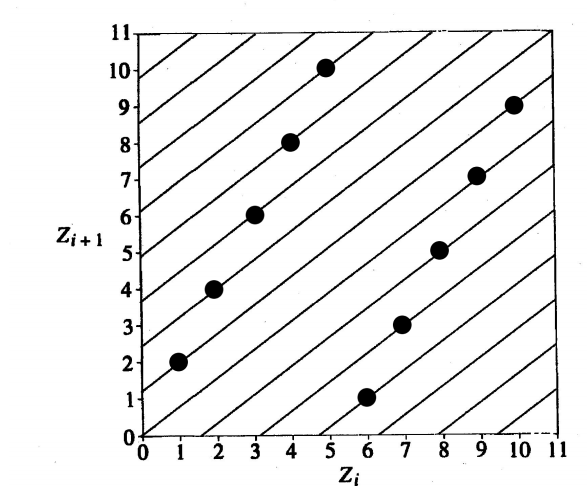
\includegraphics[width=0.2\textwidth]{assets/1.PNG}
      \end{center}
      \end{figure}
    Przez wyżej wymienione czynniki nie może być on stosowany w kryptografii.
\end{frame}
\begin{frame}
  \frametitle{Własny generator}
  Przed zaimplementowaniem pozostał jeszcze wybór $m$ oraz $a$ dla naszego generatora.

  Niech $m=2^{32}$, jest to liczba o 1 większa od zakresu unsigned int'a, dzięki czemu nasza kongruencja potencjalnie będzie mogła zwracać wszyskie liczby które jesteśmy w stanie zapisać na 4 bajtach float'a w większości języków programowania. Ponadto niech $a=747796405.$
  \begin{figure}[h]
    \begin{center}
    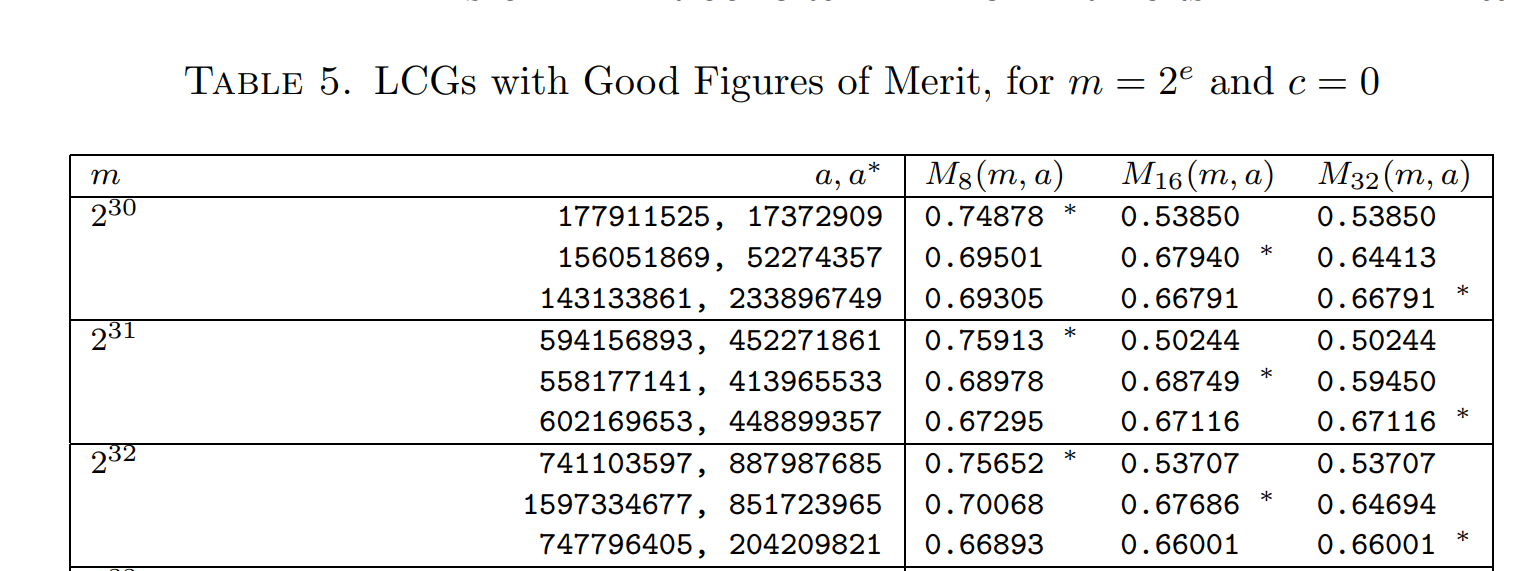
\includegraphics[width=0.7\textwidth]{assets/table.PNG}
    \end{center}
    \end{figure}
\end{frame}
\section{Własny generator - kod źródłowy}
 \begin{frame}[containsverbatim]
  \frametitle{Własny generator - kod źródłowy}
   \begin{lstlisting}[language=Python, caption=Klasa generatora]
    class generator:

        def __init__(self, seed):
            self.value = seed
            self.a = 747796405
            self.m = 4294967296

        def generateRandom(self):
            self.value = (self.a*self.value) % self.m
            return self.value
    \end{lstlisting}
    Klasa generatora posiada konstruktor który jako argument przyjmuje ziarno czyli dowoloną liczbę początkową która rozpocznie budowanie pseudolosowy ciąg. Jest także metoda która zwaraca kolejną wygenerowaną liczbę.
\end{frame}
\section{Modyfikacje generatora dla uzyskania zadanych rozkładów}
\begin{frame}[containsverbatim]
  \frametitle{Rozkład jednostajny}
  Aby uzyskać liczby z rozkładu jednostajnego na przedziale $[0,1]$ wystarczy podzielić przez ustalone wcześniej $m=4294967296$, zauważmy że po takiej operacji największą liczbą możliwą do uzyskania będzie 1, natomiast pozostałe liczby będą należały to przedziału $[0,1]$.
  \begin{lstlisting}[language=Python, caption=Metoda rozkładu jednostajnego]
    def uniformDistribution(self):
        return self.generateRandom()/self.m
    \end{lstlisting}
\end{frame}
\begin{frame}[containsverbatim]
  \frametitle{Rozkład Bernoulliego}
  Rozkład Bernoulliego, jest rozkładem dwupunktowym, aby uzyskać ten rozkład skorzystam z metody którą przygotowałem dla rozkładu jednostajnego. Ustalmy dowolne $P\in [0,1]$. Jeśli wylosowana liczba przez metodę rozkładu jednostajnego będzie mniejsza od p to zwrócimy 0, w przeciwnym razie 1.
  \begin{lstlisting}[language=Python, caption=Metoda rozkładu Bernoulliego]
    def bernoulliDistribution(self, probability):
        rand = self.uniformDistribution()
        if ( rand<= probability):
            return 0
        else:
            return 1
    \end{lstlisting}
\end{frame}
\begin{frame}[containsverbatim]
  \frametitle{Rozkład Dwumianowy}
  Rozkład dwumianowy jest to liczba sukcesów w $n$ próbach Bernoulliego. W implementacji wykorzystałem wcześniej przygotowaną metodę generowania próby Bernoulliego, wywołanie jej $samples$ razy daje nam rozkład Dwumianowy
  \begin{lstlisting}[language=Python, caption=Metoda rozkładu Dwumianowego]
    def binomialDistribution(self,probablity, n):
        counter = 0
        for i in range(n):
            counter+=self.bernoulliDistribution(probablity)
        return counter
    \end{lstlisting}
\end{frame}

\section{Sources}
\begin{frame}
  \frametitle{Sources}
  \begin{itemize}
    \item \url{http://home.agh.edu.pl/~chwiej/mn/generatory_16.pdf}
    \item \url{https://pl.wikipedia.org/wiki/Generator_liczb_pseudolosowych}
    \item \url{https://eduinf.waw.pl/inf/alg/001_search/0022.php}
    \item \url{https://www.ams.org/journals/mcom/1999-68-225/S0025-5718-99-00996-5/S0025-5718-99-00996-5.pdf}
  \end{itemize}
\end{frame}
\end{document}